\documentclass{article}
\usepackage{hyperref}
\usepackage{minted}

\usepackage[utf8]{inputenc}
\usepackage{geometry}
\usepackage{amssymb}
\usepackage{amsmath}
\usepackage{amsfonts}
\usepackage{enumitem}
\usepackage{graphicx}
\usepackage{booktabs}
\usepackage{float}
\usepackage{tikz}
\usepackage{tabularx}
\usepackage[scr]{rsfso}
% \usepackage{newpxtext,newpxmath}
\usepackage{color}
\usepackage{fullpage}
\usepackage{mathpartir}
\usepackage{multirow}

\newcounter{problemcounter}

\newcommand{\problem}[1][]{\stepcounter{problemcounter}\section*{Problem \theproblemcounter #1}\vspace{-1em}\rule{\textwidth}{1pt}
	\vspace{.25em}
}

\newcommand{\answer}[1]{\color{blue} {\bf Answer:}\\ #1 \color{black}}


\newcommand{\equivalence}[2]{#1 & \Leftrightarrow & #2}

\newcommand{\red}[1]{{\color{red} #1}}

\newcommand{\blank}[1]{\red{#1}}

\usepackage{listings}

\definecolor{codegreen}{rgb}{0,0.6,0}
\definecolor{codegray}{rgb}{0.5,0.5,0.5}
\definecolor{codepurple}{rgb}{0.58,0,0.82}
\definecolor{backcolour}{rgb}{0.95,0.95,0.92}

\lstdefinestyle{mystyle}{
    backgroundcolor=\color{backcolour},   
    commentstyle=\color{codegreen},
    keywordstyle=\color{magenta},
    numberstyle=\tiny\color{codegray},
    stringstyle=\color{codepurple},
    basicstyle=\ttfamily\footnotesize,
    breakatwhitespace=false,         
    breaklines=true,                 
    captionpos=b,                    
    keepspaces=true,                 
    numbers=left,                    
    numbersep=5pt,                  
    showspaces=false,                
    showstringspaces=false,
    showtabs=false,                  
    tabsize=2
}

\lstset{style=mystyle}



% needed to get figure counter correct
\numberwithin{figure}{section}

\title{ECE 569 Fall 2025 Lab 3}

\begin{document}

%\maketitle

\noindent
\begin{tabularx}{\linewidth}{|p{2.65in}|X|}
\hline
	\begin{minipage}{\linewidth}
	~\\
	
	{\Large ECE 569} \\
	{\bf Lab 3: Processing MoCap data} \\
	{Due Saturday, October 25th, 2025}	
	~\\
	\end{minipage}
	&
	\begin{minipage}{\linewidth}
	{\bf Name:} \vspace{0.5em} \\
	List anyone you have collaborated with:
	\\
	~\\	
	\end{minipage}
\\
\hline
\end{tabularx}

\section*{GitHub Migration}

Because of the problems with the github.itap.purdue.edu github enterprise servers, we have made Lab 3 available on a public github page, which you can access \href{https://github.com/purdue-ece569-fall2025/Lab3)}{here}.
\begin{itemize}
    \item If you have a github.com account (personal or school email) you can use it.
    \item If you do not have a github.com account, you may create one with your personal email or purdue email.
    \item You are not required to add \verb|purdue| to your username in either case.
\end{itemize}

In any case, you should add your TA \verb|Logan Dihel| as a collaborator to Lab 3 repository (username is \verb|logdog|), and you need to type your github username here \textcolor{blue}{replace me with your github username}. This is so that your TA can check your code when you are finished with the lab.

\subsection*{Step by Step Instructions for GitHub setup}
\begin{enumerate}
\item Create an account at github.com. You may need to add your Purdue email to your GitHub account (you can associate multiple emails with a single account, and you can remove the purdue email later).
\item Go to \href{https://github.com/purdue-ece569-fall2025/Lab3}{Lab 3} and press "Use this template". Make sure that the visibility is set to \textbf{private}. (It will default to public so make sure you change it!)
\item Go to your Profile Settings on github. (In top right corner, click on your avatar picture, then Settings.)
\item Click SSH and GPG keys
\item \textbf{If you are using eceprog: } Create a new SSH key called eceprog (or similar) and paste in your public key which is in eceprog. To obtain this public key, go into eceprog and run \verb|cat ~/.ssh/id_ed25519.pub| from the terminal. Copy this entire line (it will start with \verb|ssh-ed25519| and end with \verb|@purdue.edu|); this is what you need to paste into the SSH key in your github settings.
% repeat the previous number
\item[\theenumi.] \textbf{If you are not using eceprog: } Create a new SSH key and paste in your public key. To obtain this public key, run \verb|cat ~/.ssh/id_ed25519.pub| from the terminal and copy the output (it will start with \verb|ssh-ed25519| and end with \verb|@purdue.edu|). If this file does not exist, you will need to run \\
\verb|ssh-keygen -t ed25519 -C "your_email@purdue.edu"| first.
\item Clone the repository on eceprog (or your personal machine) with \verb|cd ~/ece569-fall2025| and \\ \verb|git clone git@github.com:<username>/Lab3.git|
\item You might see a message "the authenticity of host github.com can't be established... are you sure you want to continue connecting?" Type \verb|yes| and hit enter. The repo should download.
\item To verify you have push access, edit the \verb|Lab3/README.md| file, save it, and then do the git add, git commit, and git push operations to push this commit to github.com server. You can then refresh your browser to verify you were able to make the change.
\item At this time, be sure to add your TA as a collaborator. (Settings -> Collaborators -> Add people -> logdog)
\end{enumerate}

\section*{Introduction}
In this lab, you will learn to use motion capture data to reconstruct the trajectory of a rigid body in the special orthogonal group SO(3). In Step 1, you will write MATLAB (or Python) code which generates various figures (e.g., position, velocity, etc.) from motion capture data of a flapping wing robot called Metafly. In Step 2, you will use RViz to visualize the flight of the Metafly, and learn a lot about the tf2 package.

Just like the previous labs, you should make your own copy of this Overleaf file, and then replace the screenshots with your own as you go. There is one question in this lab which will require you to type your math equation in LaTeX.

\subsection*{Background}
In many cases, we may want to learn about the ground truth position and the orientation of the robot. This can be certainly done by measuring the configuration of your robot in the Motion capture system. The infrared cameras are used to identify the location of the reflective markers on the robot. The three markers are on the Metafly (flapping wing vehicle) robot as shown in the figure below.
\begin{figure}[th!]
    \begin{center}
    \includegraphics[scale=0.5]{introduction_figures/hw5_1_marker_v1.png}
    \caption{Picture from Metafly with three reflective markers}
    \label{fig:metafly}
    \end{center}
\end{figure}
\\
Each camera will identify the marker positions based on their \textbf{Camera frame}. Since multiple cameras observe the same markers at different angles, each will create its perspective of the markers' locations. If we know the relative configurations (position and orientation) of each camera frame, then we can convert the coordinates with respect to each other's frame. That is cool! 
\\
\\
Even better, you don't need to know your relative position. You can use an object with the known marker position geometry (meaning I know the exact distance between all marker positions. We call this object as a \textbf{calibration bar} (Figure~\ref{fig:calibration}. All you need to do is keep moving around the bar in the Motion Capture Arena sufficiently long. The software will calculate the camera's relative configuration by solving optimization problems to fit into the rigid body motion of three points we know all the distances. 
\begin{figure}[t!]
    \begin{center}
    \includegraphics[scale=0.5]{introduction_figures/hw5_1_calibration.png}
    \caption{An example of calibration bar. The distance between the markers are predefined and registered to the MCP software.}
    \label{fig:calibration}
    \end{center}
\end{figure}
\\
\\
After the calibration is done, you need to define where the \textbf{world frame} is by setting the origin and the orientation of the fixed $\{s\}$-frame. This can also be done using \textbf{the calibration bar}, which has three markers making two orthogonal vectors. You put the calibration bar on the flat ground and manually define the orientation of the world frame.
\\
\\
\begin{figure}[t!]
    \begin{center}
    \includegraphics[scale=0.5]{introduction_figures/hw5_1_mocap.png}
    \caption{Heat map of MCP system (Vicon) showing the accuracy of the measurement.}
    \label{fig:heat}
    \end{center}
\end{figure}
\begin{figure}[t!]
    \begin{center}
    \includegraphics[scale=0.1]{introduction_figures/hw5_1_body.png}
    \caption{(top)Defining the Harvard RoboBee body in Nexus (Vicon software) based on the marker positions. (bottom) marker positions from the camera point of view.}
    \label{fig:body}
    \end{center}
\end{figure}
Once the world frame is defined based on the collective measurement from multiple cameras, you need to define your \textbf{robot's body frame} in this world frame. This can be done by placing the robot with the marker in the MCS arena. Then, you can manually set where the body frame is located relative to the markers on the robot in the software. See Figure~\ref{fig:body}.
\\
\\
We have PURT(The Purdue UAS Research and Test Facility) at Purdue. This is the largest MCS in the world (09/28/2023). Check out the website: \url{https://engineering.purdue.edu/PURT}.
\\
\\
In 2023, one of our TAs (Jeffery) visited the PURT to collect some open-loop flight data of the Metafly shown in Fig~\ref{fig:metafly}. The spec we choose to collect the MoCap data is as follows. 
\\
\\
\begin{tabular}{||c|c||}
    \hline
    \textbf{Sampling frequency} & 100 Hz \\
    \hline
    \textbf{Position output} & $p(t_i):=(x(t_i), y(t_i), z(t_i))\in\mathbb{R}^3$ in the world frame for all $i$ samples.
    \\
    \hline
    \textbf{Orientation output} &  $(r(t_i),p(t_i), y(t_i))\in\mathbb{R}^3$, roll-pitch yaw angle for all $i$ samples..
    \\
    \hline
    \textbf{Flapping Frequency} &  approximately $15$Hz
    \\
    \hline

\end{tabular}
\\
\\
\newline
Below is a quick understanding for the items in the .csv file provided: 
\begin{table}[h!]
\begin{center}
\begin{tabular}{|c|c|}
\hline
\textbf{t}     & time (s)                             \\ \hline
\textbf{x}     & x position of Metafly (spatial frame) (m) \\ \hline
\textbf{y}     & y position of Metafly (spatial frame) (m) \\ \hline
\textbf{z}     & z position of Metafly (spatial frame) (m) \\ \hline
\textbf{roll}  & \textcolor{red}{$\gamma$: fixed frame (about x axis) (deg)  }    \\ \hline
\textbf{pitch} & \textcolor{red}{$\beta$: fixed frame (about y axis) (deg) }      \\ \hline
\textbf{yaw}   &\textcolor{red}{ $\alpha$: fixed frame (about z axis) (deg)  }    \\ \hline
\end{tabular}
\end{center}
\end{table}

\noindent
Jeffery has collected the data for $800$ milliseconds, and ran the data through a low-pass filter to remove the high frequency noise. The output (.csv) file is listed on the GitHub page for Lab 3. The position output represents the origin of the body frame at each time point. The orientation output is the explicit coordinate of the body frame using Euler Z-Y-X angles (all in degrees).

\textbf{Note:} the figure below illustrates the body frame of Metafly and how the three axis of body rotation are defined. Please follow this convention for the rest of the assignment.
\begin{figure}[h!]
    \begin{center}
    \includegraphics[scale=0.7]{introduction_figures/metafly_frame.png}
    \caption{Metafly Body Frame Axes Illustration}
    \end{center}
\end{figure}

\newpage
\section*{Step 1: Creating Figures from Mocap Data}
\setcounter{section}{1}
\setcounter{figure}{0}
For Step 1, you need to use MATLAB (or Python) to generate various plots. You can download MATLAB onto your own computer MATLAB for free with a student account. Sign up for an account at \url{https://www.mathworks.com/academia/students.html} using your Purdue email. ThinLinc does not support MATLAB. If you choose to use Python, you may do your development on either ThinLinc or your own computer. If you use your computer for Python development, you will need to use pip to install necessary libraries like Matlplotlib and numpy. If you are new to MATLAB, we recommend going through the Lab 3 MATLAB Tutorial first, which you can access on \href{https://github.com/purdue-ece569-fall2025/Lab3}{GitHub}. We also recommend using a Live Script (.mlx) file for doing the homework. If you haven't used Python for interacting with matrices with the numpy library before, we recommend using MATLAB instead.

For Step 1, your figures will be graded on their quality and accuracy. \textbf{All figures must have appropriate axis labels with the correct units for full credit}. A test bench script will be provided for you, so you can test your functions and verify that they work. Please note that Step 1 is the hardest part of this lab, and it will consume the majority of your time. Step 2 is just a tutorial, and can be done independently of Step 1.

\newpage
\begin{enumerate}[label=(\alph*)]
\item \textbf{(Position)} Read the position data and plot the position data over time. Be careful to use the right units for each axis in your plot (the x-axis is in seconds, and y-axis is in meters). \textbf{You need to plot three subplots, demonstrating $x(t), y(t), z(t)$ over time (in seconds), with appropriate axes labels.}
\\
\\Hint: see the Lab 3 Tutorial for examples using the \mintinline{matlab}{subplot} function.
\\
\begin{figure}[H]
    \centering
    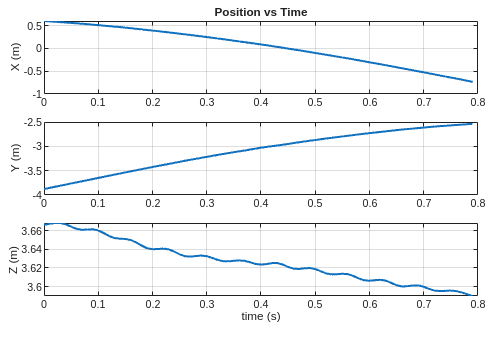
\includegraphics[width=0.75\linewidth]{Position_vs_time.png}
    \caption{Position vs Time}
    \label{fig:placeholder}
\end{figure}


\newpage
\item \textbf{(Velocity)} Using the position data, calculate the origin's velocity in the fixed frame using a first-order difference equation:
\begin{equation*}
v(t_i) = \frac{p(t_{i+1})-p(t_i)}{t_{i+1}-t_{i}}, ~~~~ i \in 1, \dots, N-1 \\
\end{equation*}
where $N$ is the number of samples from the mocap data. Since we don't have an $t_{N+1}$ sample, we can't use the first difference equation to calculate $v(t_N)$, so we just define $v(t_N) = v(t_{N-1})$. This ensures the the time array and the velocity array have the same number of entries so that we can plot velocity against time. \textbf{You need to show three subplots, demonstrating $\dot{x}(t), \dot{y}(t), \dot{z}(t)$ over time (in seconds).}
\\
\\
Hint: define a matrix $v$ where the $i$th row corresponds to the row vector $v(t_i)^\top$ and the $j$th column represents the $j$th component of $v$, indexed over all samples.
\begin{minted}{matlab}
v = zeros(N,3);
for i=1:N-1
    v(i,:) = % your code here...
end
% your code here ...
\end{minted}

\begin{figure}[H]
    \centering
    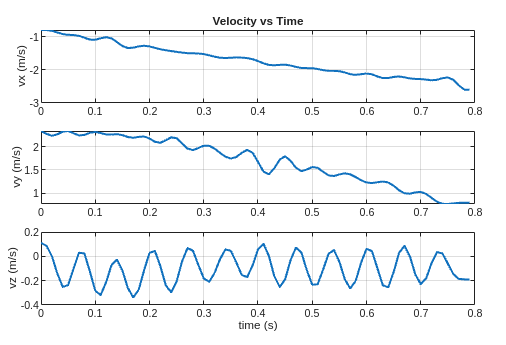
\includegraphics[width=0.85\linewidth]{Velocity vs time.png}
    \caption{Velocity vs Time}
    \label{fig:placeholder}
\end{figure}

\newpage
\item \textbf{(Orientation)} For this assignment, we will use the hat operator as defined in class.
$$\widehat\omega = \begin{bmatrix}
        0 & -\omega_3 & \omega_2 \\
        \omega_3 & 0 & -\omega_1 \\
        -\omega_2 & \omega_1 & 0
    \end{bmatrix} \in \mathfrak{so}(3)$$
We will express a rotation matrix using its exponential coordinates as
\begin{equation}
    R = e^{\widehat \omega \theta}
\end{equation}
where $\omega \in \mathbb{R}^3$ is a \textbf{unit} vector (i.e., $||\omega|| = 1$) and $\theta \in \mathbb{R}$ is a scalar. When you see $\omega$ in this assignment (as opposed to $\omega^b$), you should assume that $\omega$ is a unit vector. As a word of caution, the Modern Robotics book uses the notation $[\omega]$ to represent the hat operator, and uses $\hat \omega$ to represent a unit vector.

First, you need to implement the following three functions. Each function has already been defined with proper name, inputs, and output: you just need to fill in the body of the function with your own code. You will then test your functions by running the appropriate test bench.
\begin{enumerate}[label=\arabic*.]
\item You must implement the \textbf{ECE569\_VecToso3} (hat operator) function $f : \mathbb{R}^3 \to \mathfrak{so}(3)$ defined by the map:
$$\omega \mapsto \widehat\omega$$

\item You must implement the \textbf{ECE569\_so3ToVec} (vee operator) function $f : \mathfrak{so}(3) \rightarrow \mathbb{R}^3$ defined by the map:
$$\widehat\omega \theta \mapsto \omega \theta$$
\textcolor{blue}{
\textbf{Note:} In general, the Vee operator can take any $\widehat\omega \theta \in \mathfrak{so}(3)$ and map it into $\omega \theta \in \mathbb{R}^3$. The vector $\omega \theta$ does not need to be unit length. In your implementation, \textbf{do not} normalize the return value. 
}


\item You must implement the \textbf{ECE569\_MatrixLog3} function $f: SO(3) \to \mathfrak{so}(3)$ defined by the map: 
$$R \mapsto \widehat\omega \theta$$
\textcolor{blue}{\textbf{Note}: This is the implementation of the HW (Problem 4). Based on the conditions for the $\theta$ using the trace operation on $R$, you can explicitly find the omega. As you know the expressions are different based on $\theta$ values. You can also cross check with the expression in the Lecture note or the Section 3.2.3.3 of the Modern Robotics book. Be careful with notation!
}



\item You must implement the \textbf{ECE569\_AxisAng3} function $f : \mathbb{R}^3 \to \mathbb{R}^3 \times \mathbb{R}$ defined by the map:
$$\omega \theta \mapsto (\omega, \theta)$$
\textcolor{blue}{
\textbf{Note:} As discussed above, $\omega \in \mathbb{R}^3$ is a unit vector, and $\theta \in \mathbb{R}$ is a scalar. (Technically, we could instead write $f: \mathbb{R}^3 \to S^2 \times \mathbb{R}$ because by definition any unit vector $\omega \in \mathbb{R}^3$ can be represented as a point on the 2-sphere $\omega \in S^2$ because the 2-sphere is the set of all points in $\mathbb{R}^3$ at a unit distance from the origin, but this seems to only complicate the function definition so we will just write $\omega \in \mathbb{R}^3$ and $||\omega|| = 1$.)
}



\end{enumerate}


\textbf{MATLAB users:} please run the command \textcolor{blue}{\mintinline{bash}{runtests}} from the MATLAB Command Window. Make sure all files from Step1/MATLAB are in your current directory.

\textbf{Python users:} please run \textcolor{blue}{\mintinline{bash}{python3 tests.py}} from the Lab3/Step1/Python directory.

After you have confirmed that each of your four functions is passing the test bench, take a screenshot of the successfully run test bench. Then, you may move on to the rest of part (c). (If your functions don't work now, then the rest of Step 1 won't be possible.)

\begin{figure}[H]
    \centering
    \includegraphics[width=0.75\linewidth]{3 Runtests.png}
    \caption{Test Bench (in MATLAB )}
    \label{fig:placeholder}
\end{figure}


\newpage
We can generate $R$ from a given \textcolor{red}{roll-pitch yaw angle $(\gamma,\beta, \alpha)$} using the equation:

\begin{eqnarray*}R_{sb}^{rpy}(\alpha,\beta,\gamma)&=&Rot(z_s, \alpha)Rot(y_s, \beta)Rot(x_s, \gamma)R_{sb}=Rot(z_s, \alpha)Rot(y_s, \beta)Rot(x_s, \gamma)I
\\
&=&
    \begin{bmatrix}
        \cos{\alpha}\cos{\beta} & \cos{\alpha}\sin{\beta}\sin{\gamma}-\sin{\alpha}\cos{\gamma} & \cos{\alpha}\sin{\beta}\cos{\gamma}+ \sin{\alpha}\sin{\gamma}\\
        \sin{\alpha}\cos{\beta} & \sin{\alpha}\sin{\beta}\sin{\gamma}+ \cos{\alpha}\cos{\gamma} & \sin{\alpha}\sin{\beta}\cos{\gamma}- \cos{\alpha}\sin{\gamma}\\
        -\sin{\beta} & \cos{\beta}\sin{\gamma} & \cos{\beta}\cos{\gamma} 
        \end{bmatrix}
\end{eqnarray*}
\\

To save you time, we have calculated $R(t_i)$ for you in the starter code, expressed as an $3 \times 3 \times N$ matrix. Each matrix $R(t_i)$ can be accessed using \mintinline{matlab}{R(:,:,i)}.



Compute the exponential coordinate of the rotational matrix for every time index: $\omega(t_i)\in\mathbb{R}^3, \theta(t_i)$ for all $i$. Plot the exponential coordinates over time. \textbf{You need to show  four subplots, demonstrating $\omega_1(t), \omega_2(t), \omega_3(t), \theta(t)$ over time (in seconds)}, where $ \omega = ( \omega_1,  \omega_2,  \omega_3)$.
\\
\\
Hint: Create a $N \times 3$ matrix \mintinline{matlab}{w} where the $i$th row represents $ \omega(t_i)^\top \in \mathbb{R}^3$ and the $j$th column represents the $j$th component of $\omega$ indexed over all time. Create a $N$ vector $\theta$ to represent each $\theta(t_i)$. You already have written functions which, together, can convert $R \mapsto (\omega, \theta)$. You just need to call them appropriately and create the plots.

\begin{figure}[H]
    \centering
    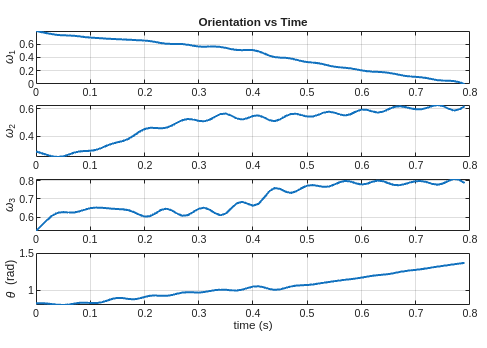
\includegraphics[width=0.75\linewidth]{Orientation vs time.png}
    \caption{Orientation vs Time}
    \label{fig:placeholder}
\end{figure}

\newpage
\item \textbf{(Angular velocity)} Now, this is a fun part where you can use your knowledge to calculate the body's angular velocity! Instead of calculating the numerical derivatives of the roll-pitch-yaw angles, we can find the angular velocity directly from the Rotational matrix $R(t_i)\in SO(3)$. This will help us to avoid any singularities caused by the roll-pitch-yaw angles. However, since $SO(3)$ is not same as the Euclidean space ($\mathbb{R}^3$), we cannot take the Euler numerical derivatives, but we can calculate \textbf{how much the frame rotates from each time sample to the next sample in the body frame}. This can be approximated by:
\begin{equation*}
    R(t_{i+1})=R(t_{i})e^{\widehat{\omega}(t_i)\theta(t_i)}
\end{equation*}
where $\omega(t_i)$ represents the (instantaneous) unit axis of rotation in the body frame at time $t_i$, and $\theta(t_i)$ represents how much angle it turned from time $t_i$ to $t_{i+1}$. Therefore, you can use the your MatrixLog3 algorithm to find $\widehat{\omega}(t_i)$ and $\theta(t_i)$:
\begin{equation*}
    \widehat{\omega}(t_i)\theta(t_i) = \log(R(t_{i})^\top R(t_{i+1}))
\end{equation*}
Then, after using the $\lor$ map (the vee map or wedge map that converts $\widehat\omega \mapsto \omega$, which you have already implemented) the angular velocity in the body frame $\omega^b$ is given by:
\begin{equation*}
\omega^b(t_i)=\omega(t_i) \dot{\theta}(t_i) \approx \frac{\omega(t_i)\theta(t_i)}{t_{i+1}-t_i}
\end{equation*}
Note: the angular velocity $\omega^b = (\omega^b_1, \omega^b_2, \omega^b_3) \in \mathbb{R}^3$ is not necessarily a unit vector. 
\textbf{You need to show  three subplots, demonstrating $\omega^b_1(t), \omega^b_2(t)$ and  $\omega^b_3(t)$ over time (in seconds)}. The last element of $\omega^b$ can be set to be the previous one, as we did with the velocity in (b) (e.g., $\omega^b(t_N)=\omega^b(t_{N-1})$).

\begin{figure}[H]
    \centering
    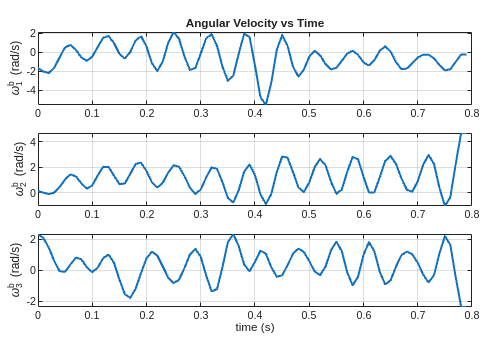
\includegraphics[width=0.75\linewidth]{Angular velocity vs time.png}
    \caption{Angular Velocity vs Time}
    \label{fig:placeholder}
\end{figure}

\newpage
\item \textbf{Error Metric on SO(3)}
Suppose that we want to understand how we can control the flying robot to make the exact attitude (orientation) in the air. Hovering vehicle is one of the ways that we want to make the body $z$-axis to be aligned with the world $z$-axis. If we want to pass the gap that is skewed, then we probably want to enter the gap with an exactly desired orientation in space. If you are interested, you can read this paper: \url{https://ieeexplore.ieee.org/ielaam/7083369/7797562/7762111-aam.pdf}, and the video can be found here: \url{https://www.youtube.com/watch?app=desktop&v=5l27chpTzhg}. 
\\
\\
Now, as a student of ECE569 class, we can ask \textbf{"how can I determine if my robot is currently at the desired orientation or not?"} This is an equivalent question to ask about \textbf{"how far is my robot currently, $R(t)$, to the desired orientation $R_d\in SO(3)$?"} In Euclidean space, it is very natural to think about the distance between two points: a straight line. Every point on the line was on the Euclidean space. Inspired by this, we can think of finding the \textbf{distance between $R(t)$ and $R_d$ in SO(3)}.
\\
\\
One way to use the distance between two orientations is by asking about what is the distance between any two square matrices?
\begin{equation}
\label{eqn:induced_norm}
    d(M_1,M_2)=||M_1-M_2||_2
\end{equation}
For $M_1, M_2\in\mathbb{R}^{n\times n}$, the $n\times n$ matrix can be viewed as a \textbf{vector in $\mathbb{R}^{n^2}$} by stacking all the columns up. Then we can use the Euclidean 2-norm for a vector in $\mathbb{R}^{n^2}$, meaning,
\begin{equation}
    ||M||^2_2 = \sum_{i=1}^{n}\sum_{j=1}^{n} m_{ij}^2 = Tr(M^\top M)
\end{equation}
where $m_{ij}$ is the i-j the element of $M\in\mathbb{R}^{n\times n}$. You may want to think carefully about why it is equal to the trace of $M^\top M$. Now, using this norm, we can define the induced metric as shown in (\ref{eqn:induced_norm}). Therefore, the distance between two square matrices can be written as 
\begin{equation}
    d(R(t),R_d)^2 = ||R(t)-R_d||^2_2=Tr((R(t)-R_d)^\top(R(t)-R_d))
\end{equation}
\begin{enumerate}[label=\arabic*.]
\item Show that 
\begin{equation}
    d(R,R_d)^2 = 2Tr(I-R^\top R_d)
\end{equation}
holds for $R, R_d\in SO(3)$. \textbf{Please type your proof in LaTeX below.}
\\
\\
\textbf{Hint}: use $Tr(A+B) = Tr(A) + Tr(B)$ and $Tr(A^\top B)=Tr(B^\top A)$)

% begin: please type your solution here
\begin{align}
    Tr((R-R_d)^\top(R-R_d)) &= something... \\
    &= something ... \\
    &= something ... (etc) \\
\end{align}
% end: please type your solution here

\newpage
\item Now, let $R_d=R(t_N)$ the last orientation of the sampled data you have. Compute $d(R(t_i), R_d)$ for all time index $i$, and \textbf{plot $d(R(t),R_d)^2$ over time (seconds)}. (Be careful, you need to plot the square of the distance).
\end{enumerate}

\begin{figure}[H]
    \centering
    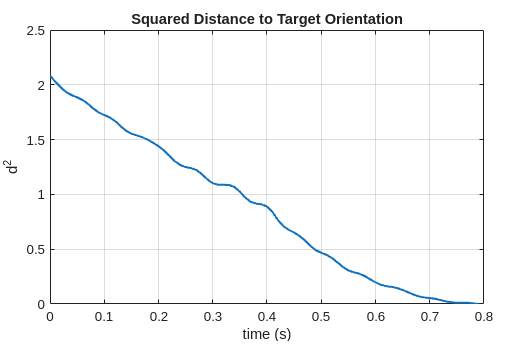
\includegraphics[width=0.75\linewidth]{Distnace square vs time.png}
    \caption{Distance Squared vs Time}
    \label{fig:placeholder}
\end{figure}

\newpage
\section*{Step 2}
\setcounter{section}{2}
\setcounter{figure}{0}
Please follow the instructions for Step 2 on GitHub. Once you have completed the tutorial, take a screenshot of the Metafly flying in RViz with the blue trail enabled. \textbf{Make sure that I can see the entire RViz window, which includes your legible username in the top.} \textcolor{red}{You will only receive credit if your username is in the screenshot as shown below.} (This is because last year, there were a few instances of screenshot sharing between students. We want to make sure students that do the work are getting the credit they deserve.) If you are using your own machine and you have different username than your Purdue email, just put this information in the caption of the image below. 
\textbf{Step 2 will be graded as Pass/Fail, so please ensure that all of the required components are in your screenshot!}

\begin{figure} [h]
    \centering
    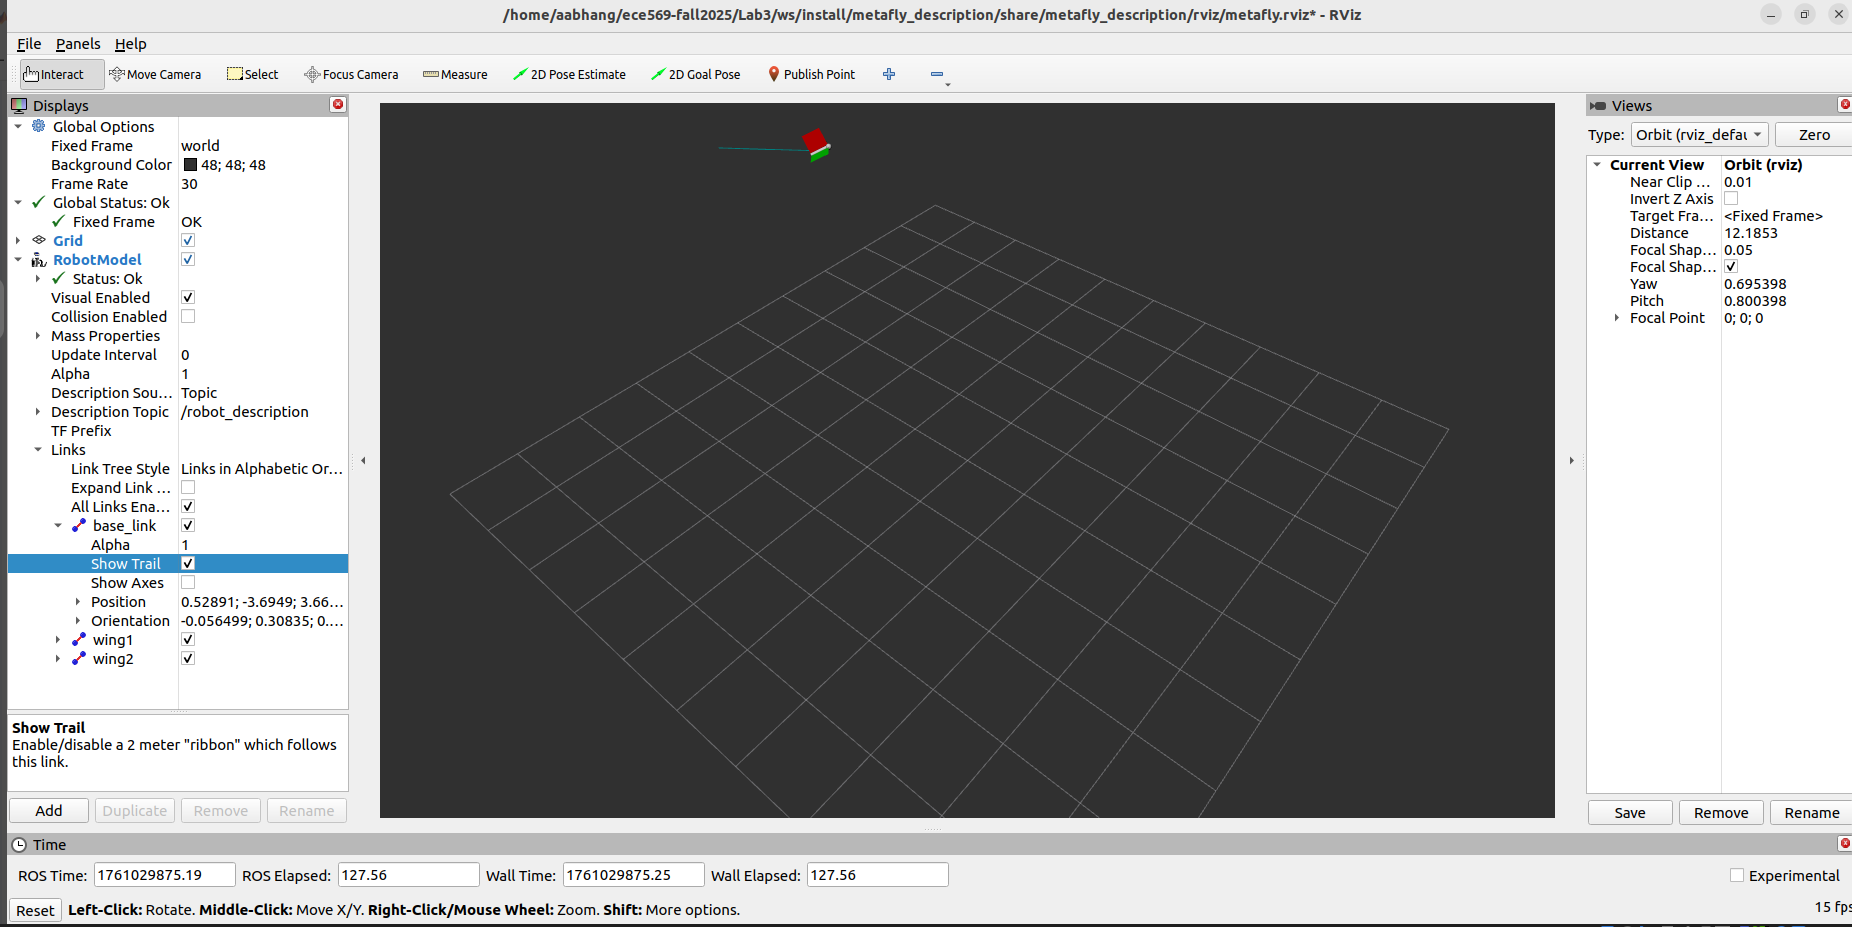
\includegraphics[width=0.95\linewidth]{Step 2.png}
    \caption{Metafly in RViz (\textcolor{blue}{My email is aabhang@purdue.edu, my username is aabhang}).}
    \label{fig:placeholder}
\end{figure}

\end{enumerate} 
\end{document}